% Compile with XeLaTeX from the outputs directory.
\documentclass[UTF8,a4paper,zihao=5]{ctexart}
\usepackage[margin=18mm]{geometry}
\usepackage{amsmath,booktabs,array,fancyhdr,graphicx}\usepackage[hidelinks]{hyperref}\usepackage{eso-pic}
\pagestyle{fancy}\fancyhf{}\renewcommand{\headrulewidth}{0pt}\fancyfoot[C]{\thepage}
\setlength{\headheight}{15pt}
\setlength{\parskip}{2pt}
\title{当代人工智能实验二：搜索算法}\author{}\date{}
\begin{document}
\AddToShipoutPictureFG*{\AtPageUpperLeft{\raisebox{-12mm}[0pt][0pt]{\hspace{20mm}\small\textbf{代码仓库：}\url{https://github.com/meltedberry/course_contemporary-ai}}}}
\maketitle\vspace{-22mm}
\section{实验目标与实现方法}
本实验围绕四个问题实现并比较 A*、Minimax 和 Alpha-beta：前两题求解单位代价与加权地形中的最优路径，第三题分析博弈树的数值回传与剪枝，第四题将路径规划与对抗搜索结合，求解宝藏分配问题。实验先核对给定样例，再通过扩大地图和博弈树规模，观察启发函数、节点访问顺序及搜索深度如何影响搜索开销。代码位于本报告目录的上一级：运行 \texttt{python experiment.py} 校验四题，运行 \texttt{python benchmark.py} 复现对照实验；环境与依赖见 \texttt{README.md}。

A* 用格点坐标表示状态，即 $n=(r,c)$，$g(n)$ 为从起点到该格的最小已知代价，用 $h(n)$ 估计剩余代价，并按 $f(n)=g(n)+h(n)$ 从小到大选择节点。用最小堆保存 $(f,g,(r,c))$，同 $f$ 时优先较小 $g$，再按坐标排序。相邻格依次向右、下、左、上生成；只有找到更小的 $g$ 时才更新记录并入堆，出堆时跳过已被更优记录替代的条目。到达终点后，沿父指针回溯得到完整路径。节点数统计有效出堆次数，包含终点；无解返回代价 $-1$ 和空路径，起终点重合返回零代价。

博弈搜索从 MAX 开始，双方轮流行动：MAX 取子节点的最大值，MIN 取最小值。Minimax 递归评估所有合法分支；Alpha-beta 在此基础上维护上下界。当某个分支已无法改善祖先的选择时，即 $\alpha\geq\beta$，便停止搜索该节点剩余的子分支。博弈节点数统计递归调用次数，包含根、内部节点与叶子；叶子数单独统计。题三默认从左到右，题四自然顺序为 T1、T2、T3、T4，反序与即时收益降序作为对照。同分保留先访问的行动。

\section{题目一：迷宫寻路}
四方向单位代价下，采用曼哈顿距离
\[
h(n)=|r-r_E|+|c-c_E|.
\]
每次移动最多使曼哈顿距离减一，故该函数不超过剩余真实代价，且满足一致性。A* 在终点有效出堆时得到最短路径。
\[
\begin{aligned}
(0,0)&\to(0,1)\to(0,2)\to(1,2)\\
&\to(1,3)\to(1,4)\to(2,4)\to(3,4).
\end{aligned}
\]
路径共有八个坐标，对应七次移动，总代价为 7。起终点的曼哈顿距离也是 7，因此该路径达到了任何可行解都无法低于的下界。具体来看，路径先到达 $(0,2)$，再向下进入第一行，绕过 $(0,3)$ 的障碍后沿最右列到达终点。
\begin{center}
\begin{tabular}{lrr}\toprule
启发函数 & 最短代价 & 扩展节点数\\\midrule
$h=0$ &7&16\\
曼哈顿距离 &7&14\\\bottomrule
\end{tabular}
\end{center}
两种方法都得到代价为 7 的路径。加入曼哈顿启发式后，扩展节点由 16 个降至 14 个，减少 $12.5\%$。这是因为偏离目标的节点通常具有更大的 $f$，会被推迟访问；对于 $f$ 相同的节点，访问顺序仍由堆的次级排序规则决定。

\section{题目二：加权地形与零代价终点}
移动代价取进入格的权值，进入 E 的代价为 0，起点不计费。输出路径为
\[
\begin{aligned}
(0,0)&\to(1,0)\to(2,0)\to(3,0)\to(3,1)\\
&\to(3,2)\to(4,2)\to(4,3)\to(4,4).
\end{aligned}
\]
沿途八次移动的代价依次为 $1,1,1,1,1,1,1,0$，累计值为 $1,2,3,4,5,6,7,7$。路径避开了高代价格；最后一次移动进入 E，不增加费用，因此八步移动的总代价为 7。

本题不能直接使用普通曼哈顿距离作为可采纳启发式：与 E 相邻的格到 E 的真实代价为 0，曼哈顿距离却为 1；起点的曼哈顿距离 8 也大于最优代价 7。设非终点格最小进入代价为 $m$，改用
\[
h(n)=m\max\{0,\|n-E\|_1-1\}.
\]
任一路径至少需要 $\|n-E\|_1$ 步，其中最后一步免费，其余每步至少支付 $m$，因此该下界可采纳。非终点间移动使启发值最多下降 $m$，进入终点时两端启发值均为 0，故它也满足一致性。本例 $m=1$。
\begin{center}
\begin{tabular}{lrr}\toprule
启发函数 & 最小代价 & 扩展节点数\\\midrule
$h=0$ &7&15\\
修正曼哈顿距离 &7&11\\\bottomrule
\end{tabular}
\end{center}
修正后的启发式与 $h=0$ 得到相同的最优代价，但将扩展节点由 15 个降至 11 个，减少 $26.7\%$。这说明设计启发函数时，必须先确定每一步的计费规则，再据此构造剩余代价的下界。

\section{题目三：博弈树求值与剪枝}
按题目 JSON 与构建代码，根的两个 MIN 子树分别为 $[[3,5],[6,9]]$ 与 $[[6,9],[1,2]]$。四个底层 MAX 的返回值为 $5,9,9,2$；MIN 返回 $5,2$，根返回 $\max(5,2)=5$。代码对重复引用的子树按每次递归分别计数。

左到右搜索时，左侧 MIN 首先得到 5，使其 $\beta=5$。接下来 MAX 读到 6 后已有 $\alpha=6\geq5$，叶子 9 被剪去：该分支最终值至少为 6，左侧 MIN 已能选择 5，后续叶子不能改变其决定。
\begin{center}
\begin{tabular}{lrrr}\toprule
方法与顺序 & 返回值 & 总节点 & 叶子\\\midrule
Minimax，正序或反序 &5&15&8\\
Alpha-beta，正序 &5&14&7\\
Alpha-beta，反序 &5&14&7\\\bottomrule
\end{tabular}
\end{center}
将每层子节点的访问顺序反转后，仍只需评估七个叶子，结果同样为 5。两种顺序建立边界的过程不同，但在这棵小树上恰好节省了相同数量的叶子。后续随机树实验进一步考察规模增大后的剪枝效果。

\section{题目四：路径代价与竞争决策}
特殊格 A、B、T 的进入代价均为 1。对六个关键位置的每一对起终点运行 A*，矩阵行列顺序均为 A、B、T1、T2、T3、T4：
\begin{center}
\begin{tabular}{c|rrrrrr}\toprule
起点/终点&A&B&T1&T2&T3&T4\\\midrule
A&0&12&10&4&8&8\\
B&12&0&8&8&4&10\\
T1&10&8&0&6&6&12\\
T2&4&8&6&0&6&6\\
T3&8&4&6&6&0&6\\
T4&8&10&12&6&6&0\\\bottomrule
\end{tabular}
\end{center}
本例矩阵对称。将一条路径反向后，中间格的费用不变，差异仅来自两个端点；六个关键点的进入代价均为 1，因此双向最小代价相同。

状态定义为 $s=(p_A,p_B,R,S_A,S_B,t)$：双方位置、剩余宝藏集合、累计收益以及当前玩家。宝藏价值为 $(9,6,7,7)$。选取 $i$ 后仅更新行动者位置并从 $R$ 删除 $i$，其分数增加 $V_i-D(p,i)$，随后切换玩家。经过其他宝藏不触发收集。

实现以未来收益差为递归返回值，累计分数作为路径上的加法项：MAX 的一步贡献为 $q=V_i-D(p_A,i)$，MIN 为 $q=-[V_i-D(p_B,i)]$。到深度零返回未来贡献 0；当前总效用等于已累计收益差加返回值。这与显式传递双方累计分数等价。递归搜索子树时将窗口变为 $(\alpha-q,\beta-q)$，返回后加回 $q$，确保剪枝界限使用同一效用坐标。
\begin{center}
\begin{tabular}{clcrr}\toprule
深度 & 方法/顺序 & 首步 & 收益差 & 节点/叶子\\\midrule
2 & Minimax，任一顺序 &T2&$-1$&17/12\\
2 & Alpha-beta，自然 &T2&$-1$&13/8\\
2 & Alpha-beta，反序 &T2&$-1$&16/11\\
2 & Alpha-beta，即时收益 &T2&$-1$&11/6\\\midrule
4 & Minimax，任一顺序 &T3&3&65/24\\
4 & Alpha-beta，自然 &T3&3&47/16\\
4 & Alpha-beta，反序 &T3&3&46/16\\
4 & Alpha-beta，即时收益 &T3&3&37/12\\\bottomrule
\end{tabular}
\end{center}
深度 2 时，A 取 T2 获益 $6-4=2$，B 取 T3 获益 $7-4=3$，收益差为 $-1$。深度 4 的一条最优应对序列为 A:T3、B:T1、A:T2、B:T4，收益依次为 $-1,1,0,-5$，最终差为 $(-1+0)-(1-5)=3$。

\section{搜索策略的对照分析}
\subsection{深度改变为何影响首步}
深度为 2 时，搜索在双方各行动一次后结束，因此选择 T2 可以得到最大的两回合收益差。深度为 4 时，搜索覆盖全部行动，既要计算当前收益，也要考虑取宝后的位置以及留给对手的选择。虽然 A 首先取得 T3 的收益为 $-1$，但在上述最优应对序列中，B 最后只能从 T1 前往 T4，承担 $-5$ 的收益。A 因而以较低的首步收益换得了更高的最终收益差。

\subsection{即时收益排序}
对每个节点，将剩余宝藏按当前行动者的 $V_i-D(p,i)$ 降序访问。MAX 较早得到高候选值，MIN 较早获得较大的自身收益，从而更快压低 A 的收益差。深度 4 时总节点由 Minimax 的 65 减至 37，减少 $43.1\%$；相对自然顺序 Alpha-beta 的 47 减少 $21.3\%$。深度 2 时节点由自然顺序的 13 减至 11。排序只改变访问顺序，三个顺序所得首步与效用一致。

\subsection{空白网格：为什么准确的启发值仍会扩展很多节点}
构造 $10\times10$、$30\times30$ 的全 1 网格，从左上角到右下角，比较同 $f$ 时小 $g$ 与大 $g$ 优先的两种规则。扩展数包含起点和终点。
\begin{center}
\begin{tabular}{crrrr}\toprule
网格 & 最优代价 & $h=0$ & 曼哈顿：小 $g$ & 曼哈顿：大 $g$\\\midrule
$10\times10$&18&100&100&19\\
$30\times30$&58&900&900&59\\\bottomrule
\end{tabular}
\end{center}
在空白网格中，$g=r+c$，曼哈顿距离为 $2(n-1)-r-c$，所有格的 $f$ 都等于最优代价 $2(n-1)$。小 $g$ 优先会先访问更浅的格点，直到最后才弹出终点；大 $g$ 优先则沿最短路径向终点推进，只扩展路径上的 $2n-1$ 个节点。因此，精确启发值可以排除更差的代价层，却不能单独决定同一代价层内的访问顺序。这组对照与第 7 节的优化采用相同机制：启发函数与同优先级节点的处理规则共同决定搜索开销。

\subsection{缓存与边界输入}
增加以 $(p_A,p_B,R,t,H)$ 为键的精确剩余效用缓存，在不剪枝的 Minimax 中使用，以免把截断边界当成精确值。四回合样例缓存命中为 0，总节点仍为 65；本次访问过程中没有重复出现相同的缓存键，因此缓存未减少搜索节点。无路地图 \texttt{S X E} 返回空路径和 $-1$；单格起终点重合返回代价 0。程序同时断言综合题两个深度的收益分别为 $-1$ 和 3。

\section{规模实验与性能分析}
\textbf{设置。}Python 3.14.6；障碍率 25\%，每个规模取 20 张可达随机图，固定种子为 $10000n+k$，不可达图跳过并保留实际种子。三种算法在同图上配对比较，所有 80 张图的路径代价均与 Dijkstra 一致。每图每算法重复 7 次，先取耗时中位数，再跨图求均值；图中节点误差棒为跨图标准差。大 $g$ 优先仅将堆键第二项改为 $-g$，首要排序仍为 $f$，保持最优性。三叉博弈树每个深度取 20 个固定种子，叶值均匀抽取整数 $[-100,100]$，逐树验证两种搜索返回值一致。

\begin{center}
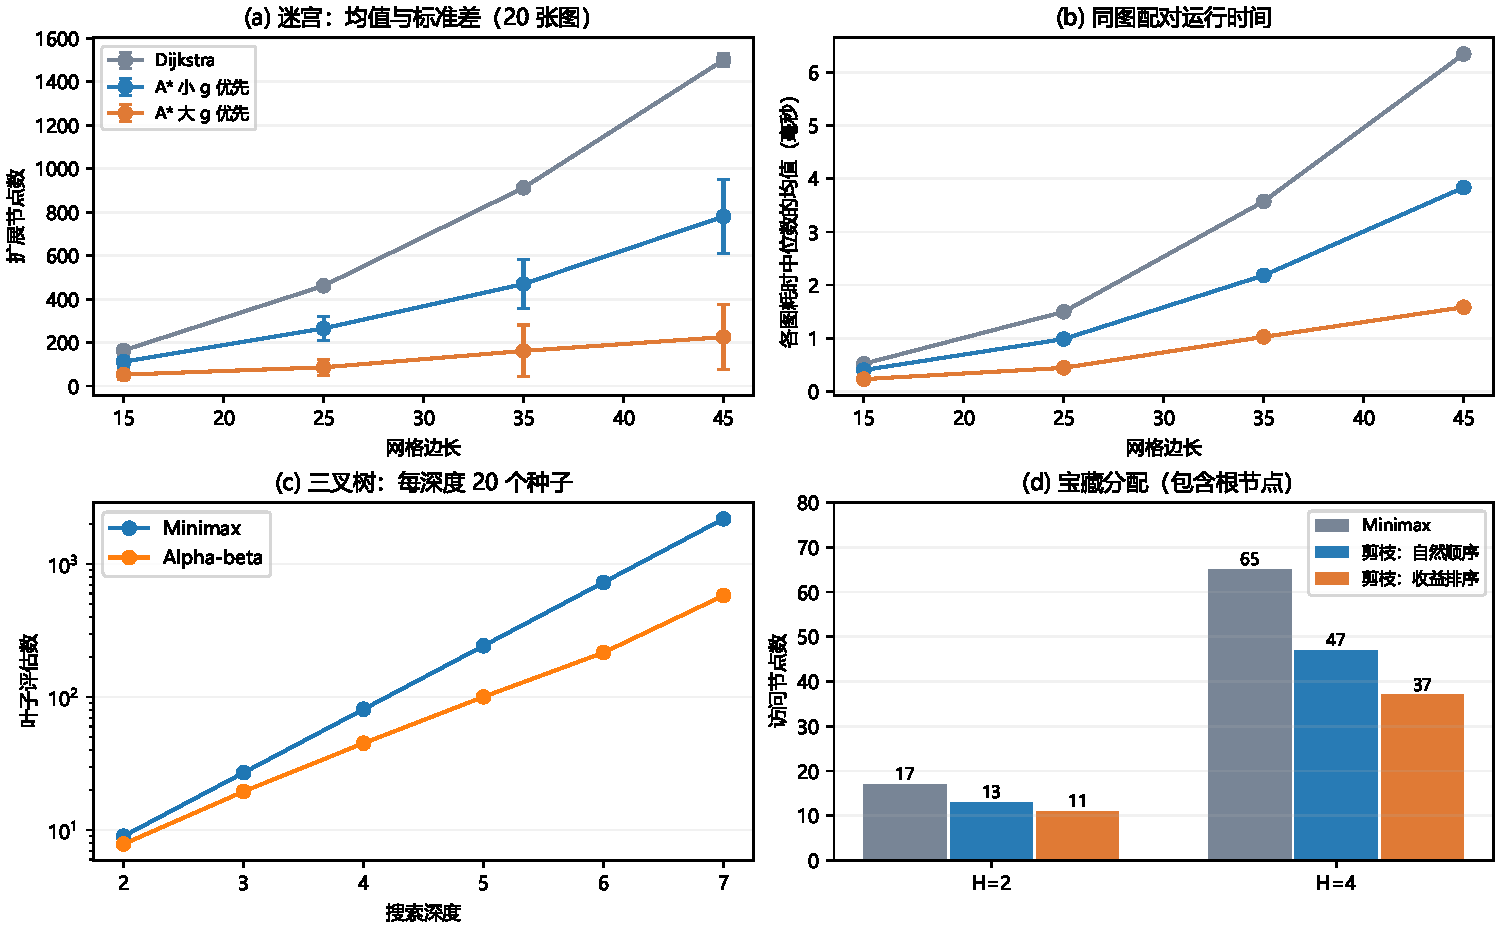
\includegraphics[width=.98\linewidth]{performance.pdf}\par
{\small 图 1\quad 迷宫、博弈树与综合题的搜索开销对照}
\end{center}
\textbf{结果。}在 $45\times45$ 上，Dijkstra、普通 A*、大 $g$ 优先 A* 平均扩展数分别为 1499.75、780.05、225.50，优化后相对基线减少 $85.0\%$；平均耗时为 6.34、3.83、1.59 ms，减少 $75.0\%$。节点收益与时间收益幅度不同，因为堆操作、邻居生成和启发值计算也占用时间。三叉树深度 7 时，Alpha-beta 平均评估 580.05 个叶子，Minimax 为 2187，减少 $73.5\%$。这些数据分别体现启发式、平局规则及剪枝对开销的影响。

\begin{center}
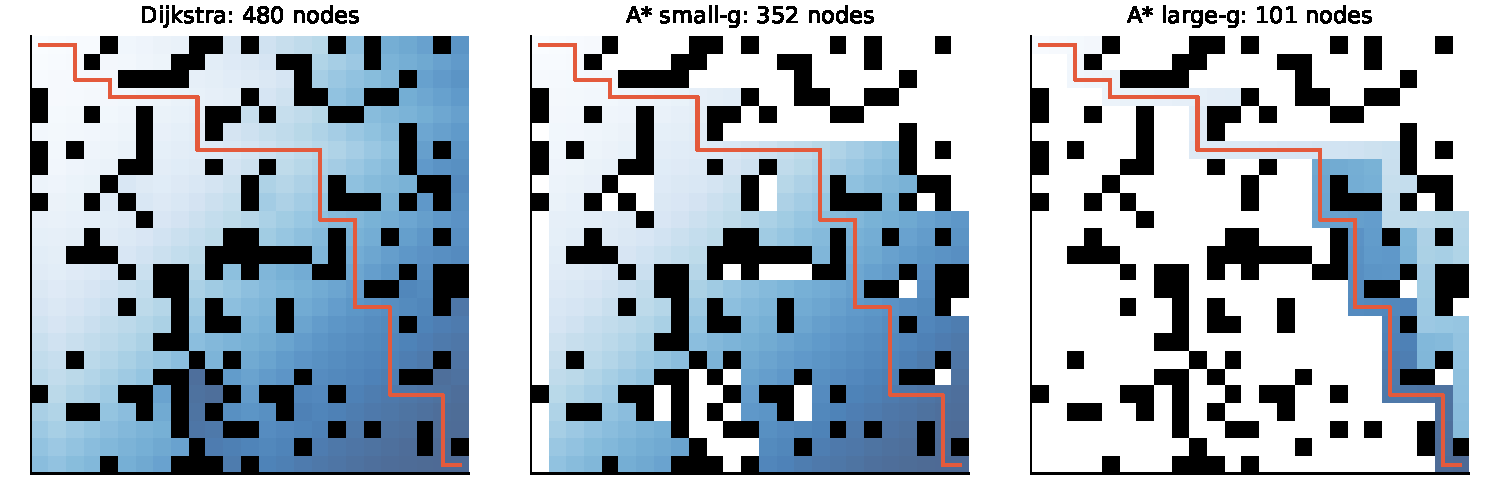
\includegraphics[width=.82\linewidth]{search_regions.pdf}\par
{\small 图 2\quad 同一地图上的搜索区域与最短路径}
\end{center}
\textbf{搜索区域。}上图选用 $25\times25$ 的第一张有效地图，黑色为障碍，蓝色为扩展格，蓝色越深表示越晚扩展，红线为最终路径。相同 $f$ 平台上，大 $g$ 优先更快向终点推进，减少横向铺展；随机图的标准差同时显示，障碍布局会改变这种收益。三种方法使用同一张地图，路径代价相同，图中的差异直接反映了节点选择策略对搜索范围的影响。

\subsection{地形感知启发式：在放宽约束的地图上求下界}
在 $31\times31$ 加权地图上（种子 20261112，障碍率 20\%，权值 1--9，终点费用为 1），先把障碍改为代价 1 的可通行格，再从终点运行反向 Dijkstra。放宽地图上的精确剩余代价作为原图的启发值：任何原图路径仍然可行，故该值不超过原图最优剩余代价；所有边代价至少为 1，因此它也不小于曼哈顿距离。实测 Dijkstra、曼哈顿与新启发式均得到代价 200，在线扩展数分别为 765、759、591，新方法比曼哈顿减少 $22.1\%$。预处理另外扩展 961 个节点，故本次单查询的总开销更高；同终点多次查询时可以复用该下界。代码与数据见 \texttt{strong\_heuristic.py} 和 \texttt{strong\_results.json}。

\section{总结}
四个给定问题均得到预期结果。路径搜索中，启发函数需要与实际移动代价一致；在满足最优性条件的基础上，同 $f$ 节点的访问顺序仍会显著影响开销。博弈搜索中，Alpha-beta 保留了 Minimax 的决策结果，行动排序进一步减少了访问节点。综合题在两个深度下选择不同首步，说明完整决策还需要考虑位置变化及后续收益。随机地图与随机树的配对实验，以及空白网格和缓存对照，共同揭示了这些策略产生收益的原因与条件。
\end{document}









